\chapter{Implementation}
\label{cha:implementation}

The vital signs Dashboard shows us different graphs with different data visualization about specific aspects of the health status of Wikipedia. Despite their overall similarity, each of them is built differently from the others due to its peculiarity.\\
In this chapter we are going to have an in-depth look at how the code is structured and at the actual implementation of each different dashboard.\\

\section{Business logic}
\label{sec:business_logic}

The main idea behind every charts is the following: we read the input from the HTML components, we process it in some way to make it compliant with the SQL queries, then we capture the outputs and feed them to the Plotly chart.\\
This whole interaction between the Dash layout and the Plotly charts is done with Dash asynchronous functions: the callbacks. Each graph has its callback that is linked to some of the HTML components and each time the user interacts with one of them, the function is called.\\
The same is done for the highlights since they also need information about the current visualization in order to adapt the captions.\\
There is also a higher level of dynamics, regarding the whole layout: in the previous chapter we have looked at an example of a Dash function that changes the layout according to the URL parameter. This whole mechanism can be described as follows:
\pagebreak
\begin{figure}[h]
    \centering
    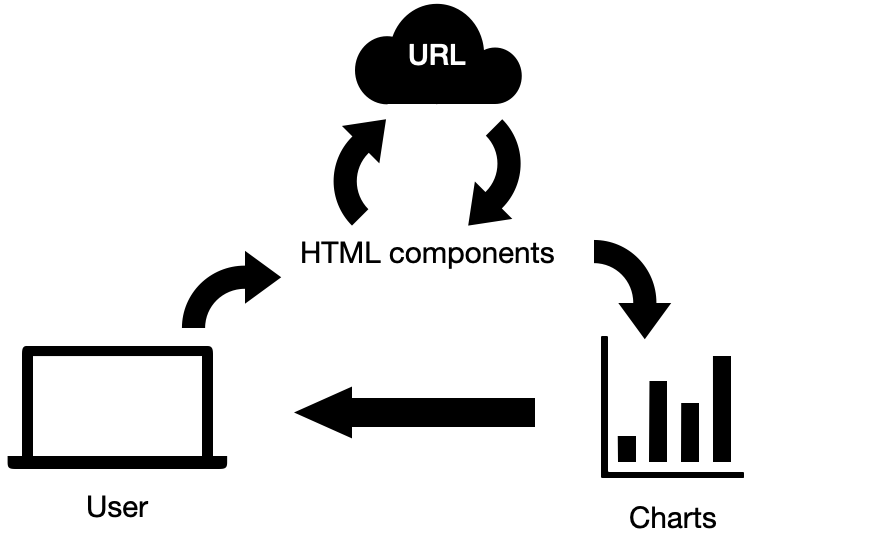
\includegraphics[width=200px]{img/callback-loop.png}
    \setlocalecaption{english}{figure}{Figure}
    \caption{Dash callback loop}
    \label{fig:callback_loop}
\end{figure}
\\
The user interacts with the HTML components, setting some parameters. When they change value, a function is activated that embed each parameter into the URL. As soon as the URL changes, a function parses it, retrieving the parameter and applying the change to the same HTML components that activated the loop. The main goal of this is that by changing the vital sign from the drop down menu, the layout is changed accordingly. Moreover, the respective vital sign callback is called, kick-starting the creation of the dashboard that will return the graph\footnote{For some vital signs there is more than one graph, even with one language only}. \\
In this way, our visualization coordinates are preserved: if we select some parameters for a certain vital sign, like Italian and French on very active editors, these choices will be maintained when we change vital sign, allowing the comparison of the same communities under different health metrics.\\
There is also another effect: by sharing our link of the current page with someone else, they will see exactly our same visualization. We remind that the goal of the project is, in fact, sharing knowledge.
We will now see each callback of the different \textit{Vital signs}.

\section{Editors}
\label{sec:editors}
The first dashboard is about editors: the users that are actively involved in the Wikipedia project by writing and editing the Wikipedia pages.\\
Based on the number of their monthly contributions we can split them into two categories: active editors and very active editors.\\
Active editors are the users that edit at least five times per month, while very active editors are those who edit at least 100 times per month.\\
From the graph in Figure \ref{fig:editors} we see the number of active and very active editors in different language communities. Since we are interested into seeing how these numbers changed over time, a line chart is provided.\\
We are also interested into comparing these values across different languages. In fact, the graph allows the visualization of different contemporary traces representing the evolution of the number of editors in different languages (with different colors).

\begin{figure}[h]
    \centering
    \includegraphics[width=470px]{img/active_editors.png}
    \setlocalecaption{english}{figure}{Figure}
    \caption{Active editors dashboard}
    \label{fig:editors}
\end{figure}

%\includegraphics[scale=0.4]{active_editors.png}

\subsection{Editors implementation}
\label{sec:editors_callback}

The Active editors dashboard is perhaps the simplest one.\\
The graph directly reads which information to display from the interactive components `` ``Language",  ``Editors" and ``Time aggregation".\\
First, the function reads the language into a list. Then, the whole languages names like ``Italian (it), German (de)" are converted through a dictionary, called \verb#language_names# into their respective language codes, to make it compliant with the SQL queries. Furthermore, an additional string is created called \verb#params#. This string is very important because in the final query we will search the languages contained in this parameter. We have obtained our first parameter.\\
We proceed to capture the type of editors the user wants to visualize. This can be done by simply filtering the input number called \verb#user_type#. If it is equal to five, then they are active editors, otherwise they are very active editors. In reality, the input number will be passed to the query untouched, since the HTML component has a numeric value behind the literal label. This is our second parameter.\\
Finally, we want to know if to display a monthly charts or a yearly one, and the process is identical to the one described for the numeric value of the editors.\\
Now, after having collected these three parameters, we can build a parameterized query by having a fixed statement and inserting, in the string, the variables containing the parameters. We then run the query to the database using pandas, yielding a data frame containing the desired information. This object is now passed to the actual plotly charts at creation time.\\

\lstset{frame=lines}
\lstset{label={lst:code_direct}}
\lstset{basicstyle=\footnotesize}
\lstset{caption=Creating a line chart}
\begin{lstlisting}

fig = px.line(
             dataframe=df,
             x='year_month',
             y='m1_count',
             color=df['language_name'],
             height=500,
             width=1200,
             title=incipit+' Users',
             labels={
                     "m1_count": incipit+" Editors ",
                     "year_month": time_text,
                     "language_name": "Projects",
                 },
            )
    
\end{lstlisting}

From the example above we can see the code responsible for the creation of a line chart. It is done using plotly express, the sub-module of plotly.\\
We can also see how we specify the data source, the data frame, and which data column we want to put on the x-axis and on the y-axis.\\
We can also see some other keywords that are useful to improve the visualization of the graph: we can set a title to enhance its readability, we can specify its size and we can also create a map that provides more readable labels for the data columns.\\
Finally the dashboard is ready to be deployed.

\section{Retention}
\label{sec:retention}

The first vital sign is Retention and it measures the percentage of new editors that survives 60 days\footnote{Retention period is not fixed but can be chosen from different time periods: 24 hours, 30, 60, 365 and 730 days} after the first edit. Survivors are meant as those users which keep editing after the time threshold. We are interested in the capability of a certain community of keeping its editors engaged, in order to understand if and why editors are leaving Wikipedia.\\
In this dashboard we can see the retention rate of one or more language communities, along the timely distribution of the registered users. From Figure \ref{fig:retention}, we can see that the graph is actually a dual-axis chart: on the left y-axis, as bars, we have the number of registered editors, while on the right y-axis we have the retention rate displayed as an orange line.

\begin{figure}[h]
    \centering
    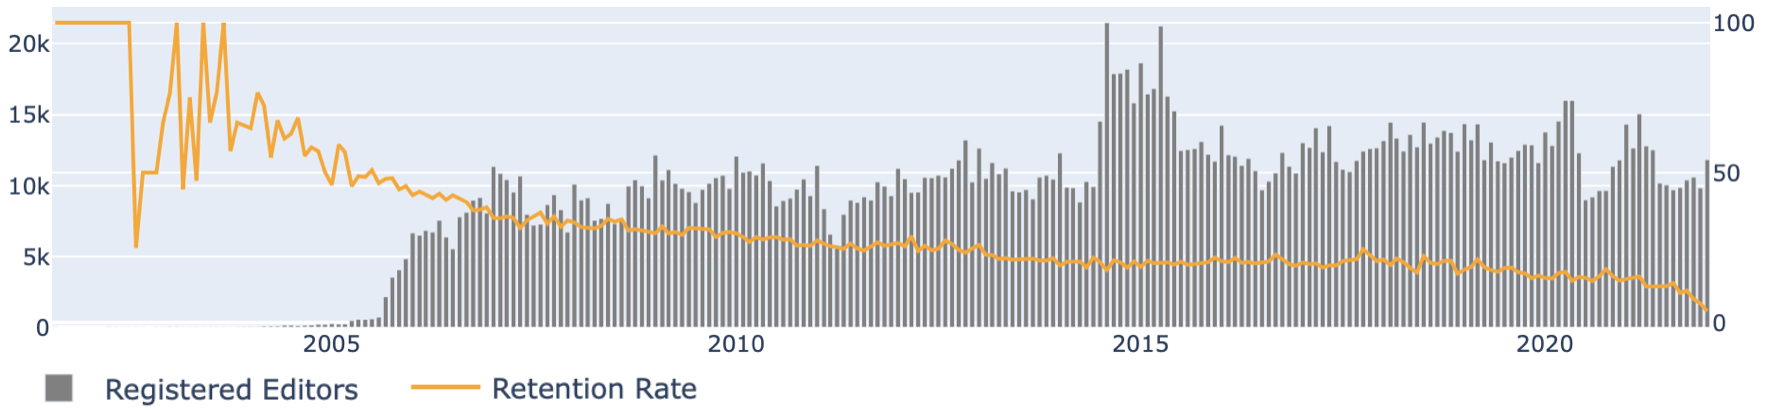
\includegraphics[height=140px, width=480px]{img/retention.png}
    \setlocalecaption{english}{figure}{Figure}
    \caption{Retention dashboard}
    \label{fig:retention}
\end{figure}

\subsection{Retention implementation}
\label{sec:retention_callback}

The retention dashboard is quite different from the previous dashboard and from the following ones since it is not a normal chart, but a dual chart.  Due to the high-level nature of plotly express, this module was not useful to code a dual-axis chart. Thus, the graph objects module was used; in particular the \verb#make_submodule()# method.

\lstset{frame=lines}
\lstset{label={lst:code_direct}}
\lstset{basicstyle=\footnotesize}
\lstset{caption=Creating a dual axis: line chart and bar chart}
\begin{lstlisting}

fig = make_subplots(
    specs=[[{"secondary_y": True}]])

fig.add_bar(
    x=df1['year_month'],
    y=df1['m1_count'],
    name="Registered Editors",
    marker_color='gray')

fig.add_trace(
    go.Scatter(
        x=df2['year_month'],
        y=df2['retention'],
        name="Retention Rate",
        hovertemplate='%{y:.2f}%',
        marker_color='orange'),
        secondary_y=True)
    
\end{lstlisting}

Here we can see the code responsible for the realization of the Retention dual axis. \\
First we create a figure with a secondary vertical axis. Then, we set which type of charts will populate this figure: we add a bar chart, for registered editors, and a line chart, for the retention rate, with \verb#go#. To enhance the readability of the latter, we use the keyword \verb#hovertemplate# to show the retention values when the cursor passes over the line.\\
We remind that our goal is to visualize Wikipedia communities health values and to compare them. In fact, when we select multiple languages in the drop down menu, one Retention graph for each language will appear. This feature is similar to the one of the following graph, but from the back-end prospective it is fundamentally different.\\
We will later discuss the use of a fundamental keyword, \verb#facet_row#, but for our current understanding we can limit to the fact that the mechanism of the Retention graphs is unlike the others.\\
To duplicate the Retention graphs based on the number of input languages, a for loop has been applied: when we dynamically return the layout, we also call the function related to that vital sign and, in this case, we return more than one retention graph, each one with a different language from the input.

\lstset{frame=lines}
\lstset{label={lst:code_direct}}
\lstset{basicstyle=\footnotesize}
\lstset{caption=For-loop to return multiple charts}
\begin{lstlisting}
array=[]
res = html.Div(children=array)

for x in language:
    fig=retention_graph(x, retention_rate, len(params))
    array.append(fig)

return res
\end{lstlisting}

In this way we by-pass the problem of \verb#go# not supporting the \verb#facet_row# keyword. We simply create multiple graphs and we return it all, yielding the visualization in Figure \ref{fig:multiple_retention}.

\begin{figure}[h!]
    \centering
    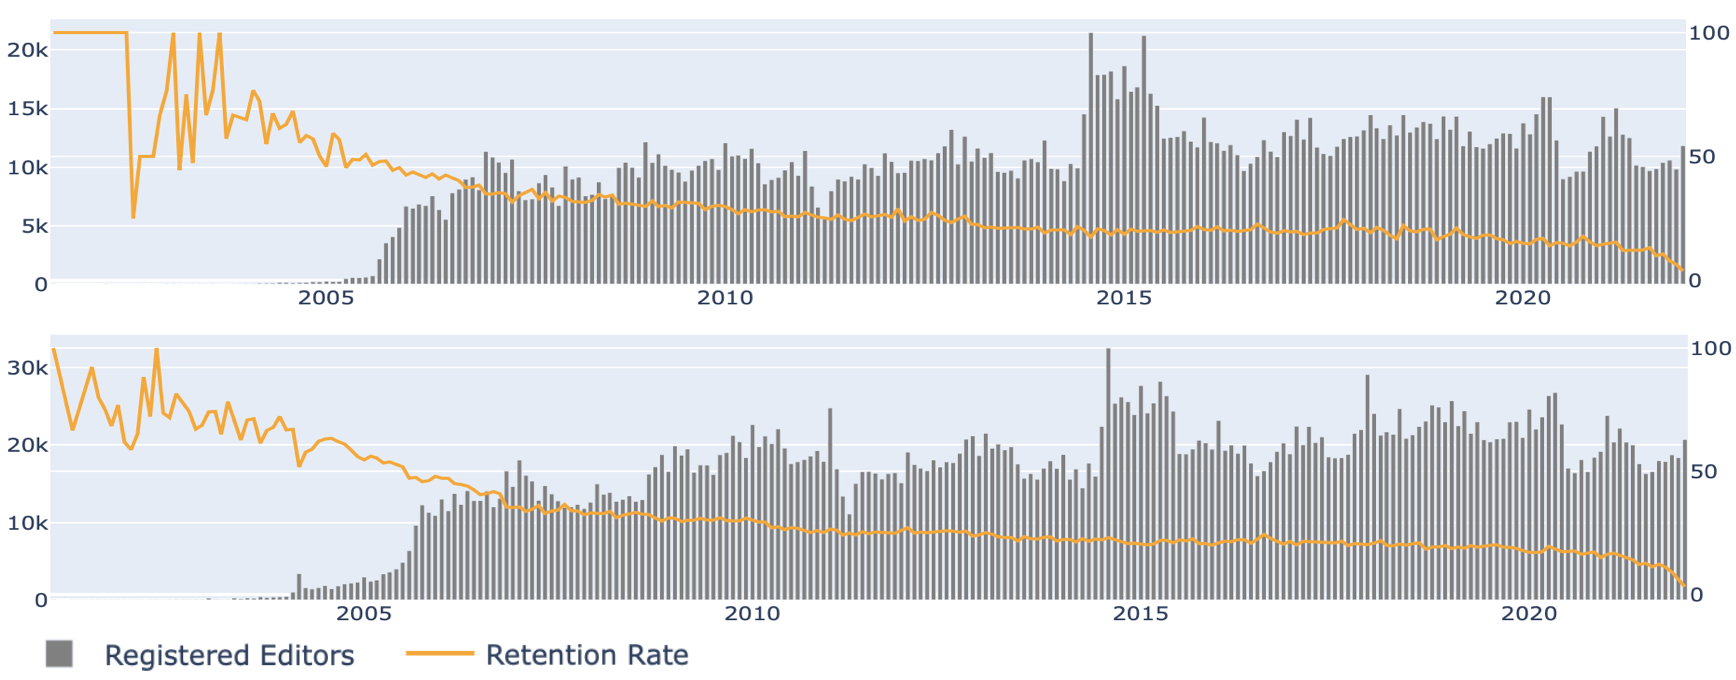
\includegraphics[width=470px]{img/multiple_retention.png}
    \setlocalecaption{english}{figure}{Figure}
    \caption{Multiple retention rates}
    \label{fig:multiple_retention}
\end{figure}

In Figure \ref{fig:multiple_retention} we can see an example of the retention graphs when multiple language are selected, in this case Italian and German.\\
This method has some drawbacks though: mainly, the visualization is not as compact as it would be with the \verb#facet_row# method, in fact the titles and the legends are repeated.

\section{Stability}
\label{sec:stability}

The second vital sign is Stability and it measures persistence of active and very active editors, as well as by the succession of the various generations of editors over time. It is a useful indicator since we want to know if a certain language community is able to attract new editors, called "fresh", and at the same time if it has solid community composed by long-term engaged editors.\\
For this metric it is convenient to classify the editors based on the number of months for which they kept editing Wikipedia's pages. We have different bin from one month to more than 24 months. The editors that keep editing for one month in a row are defined as ``fresh editors".\\
In the stacked bar chart below we can see that each bin of continuous activity is colored differently.

\begin{figure}[h]
    \centering
    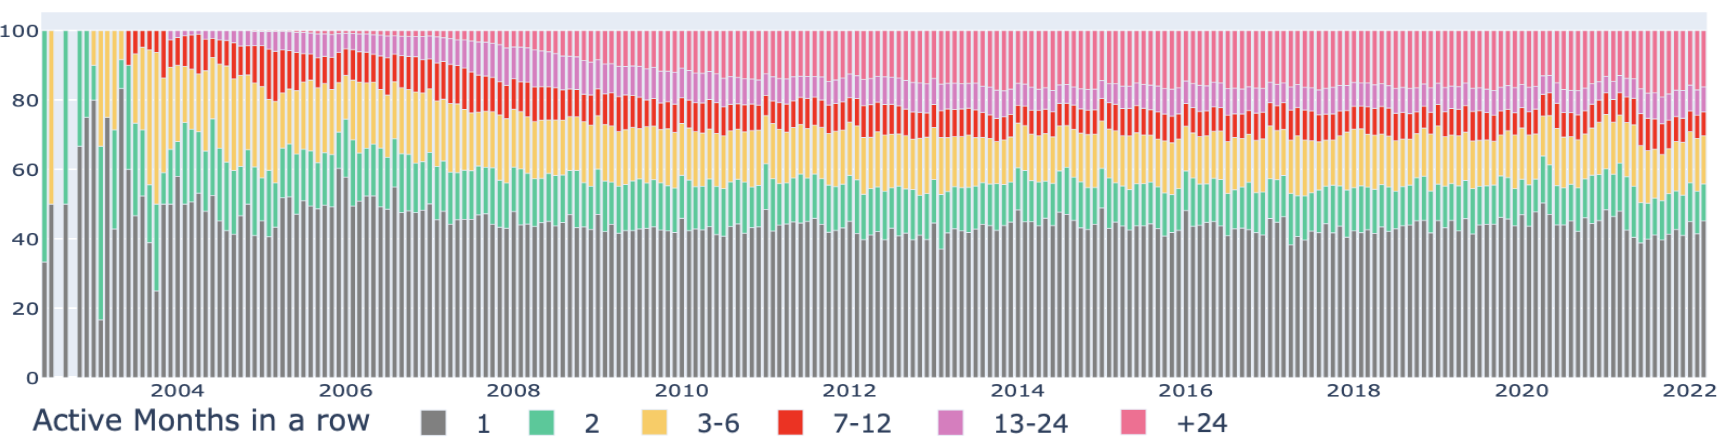
\includegraphics[width=460px]{img/stability.png}
    \setlocalecaption{english}{figure}{Figure}
    \caption{Stability dashboard}
    \label{fig:stability}
\end{figure}

The persistence of each class of editors is represented in percentage, but it could be shown by absolute values as well, through the radio buttons of the HTML components.\\

\subsection{Stability implementation}
\label{sec:stability_callback}
The stability metric is the one that introduces the most common graph in the dashboards: the stacked bar chart.\\
Despite it being different from the line chart, this type of visualization has been realized in a very similar way. First, we query the data from the database, reading the input parameter for the languages, the type of editors that can be active or very active, and the type of value that we want to see, percentage or absolute. This parameter, called \verb#value_type#, will not be included in the query, but it is necessary for the correct visualization of the chart: if the user wants to have the absolute values, nothing happens; on the other hand, for a percentage view we have to create a new data column by dividing the number of a given class of editors by the total number of editors in that month.\\
After having retrieved the data, we create the final plot using the Plotly Express \verb#px.bar()# method.

\lstset{frame=lines}
\lstset{label={lst:code_direct}}
\lstset{basicstyle=\footnotesize}
\lstset{caption=Creating a stacked bar chart}
\begin{lstlisting}
fig = px.bar(df,
             x='year_month',
             y=value_type,
             color='m2_value',
             text=value_type,
             facet_row=df['language_name'],
             width=1200,
             height=height_value,
             color_discrete_map={"1": "gray",
                                 "2": "#00CC96",
                                 "3-6": "#FECB52",
                                 "7-12": "red",
                                 "13-24": "#E377C2",
                                 "24+": "#636EFA"},
             labels={"year_month": time_text,
                     "m2_value": "Active Months in a row",
                     "m2_count":  incipit+" Editors"})
\end{lstlisting}
 %the color map and facet_row
We can observe two important keywords: \verb#color_discrete_map# and \verb#facet_row#.
With the first one we set a dictionary that maps our data column to specific colors, in order to have the full control on the final visualization. In this example it is important to avoid using similar colors in order to ensure the contrast between each editor class.
The mapping can be seen in the legend on the right in Figure \ref{fig:stability}.
The second keyword, \verb#facet_row#, is essential for the dashboards. We previously talked about this keyword in retention, explaining how we mimed its mechanism with a for-loop. \\
The \verb#facet_row# attribute \footnote{ facet row is an attribute specific of Plotly express} allows us to set a data column from the data frame, in order to multiply the graph based on each different value of that column. In this example and in the majority of the dashboards we use the \verb#langcode# data column. In this way, we will have a different visualization for each input language, allowing the comparison of the vital signs across the language communities. A meaningful milestone for the WikiCHM project.\\
\\
In Figure \ref{fig:multiple_stability} below, we can observe the result of the
so called ``faceted graph" that yields a more compact view than the for-loop method: for example, there is only one legend for all the charts and each of them is identified by the language on the right.\\
We can also observe that the size of the two graphs is smaller compared to the previous Figure \ref{fig:stability}. This is due to the fact that having many languages, thus many different graphs at their maximum size, would rapidly crowd the page in a way that would prevent making comparison between the languages at the top and the ones at the bottom. We in fact decided to dynamically reduce the size of the graphs, preventing them from becoming too small to be analyzed. However, a maximum of five languages at a time is recommended.

\begin{figure}[!h]
    \centering
    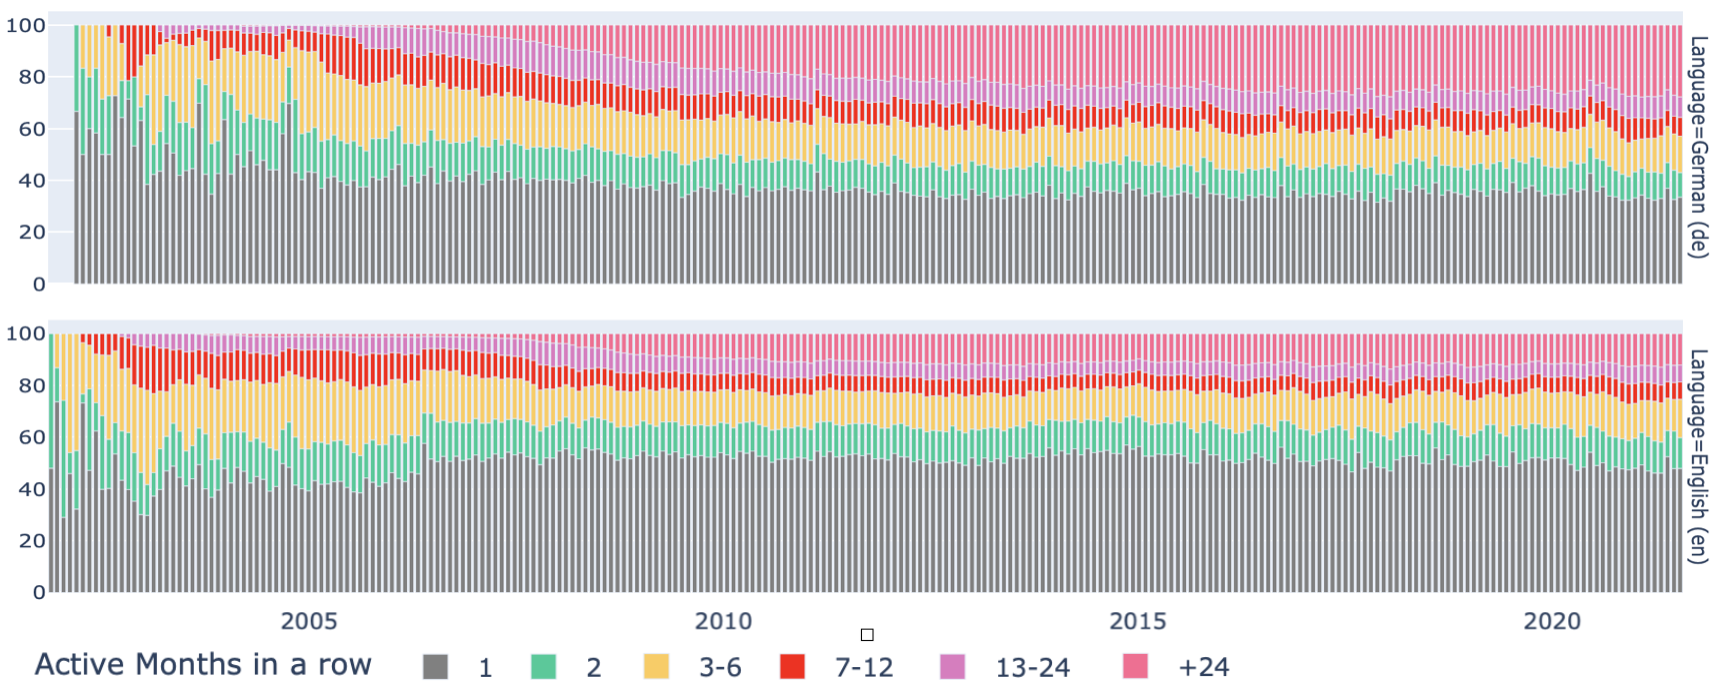
\includegraphics[width=470px]{img/multiple_stability.png}
    \setlocalecaption{english}{figure}{Figure}
    \caption{Faceted stability}
    \label{fig:multiple_stability}
\end{figure}

\section{Balance}
\label{sec:balance}

The third vital sign is community Balance. It measures the ability of a certain community of maintaining an equal proportion of old and new contributors. Previously, in stability, we monitored the distribution of some community's editors. This time, we measure the interaction of the community towards the editors, in particular how well a certain language manage the phenomenon known as ``generational change". For a better understanding of this metric, it is useful to define the concept of "generation of editors": a generation is considered to be five years. This time we discriminate the editors based on their temporal belonging, not on their continuous contribution.\\
In this visualization we can see different colors representing the different generations, from the birth of Wikipedia until our current days (and beyond).
The stacked bar chart is very convenient: for a given year, or month, we can observe the actual distribution of different generation of user, enabling the possibility of doing quantitative analysis. As was said before, the metrics support absolute and percentage values. In this case, a percentage visualization is recommended.

\begin{figure}[h]
    \centering
    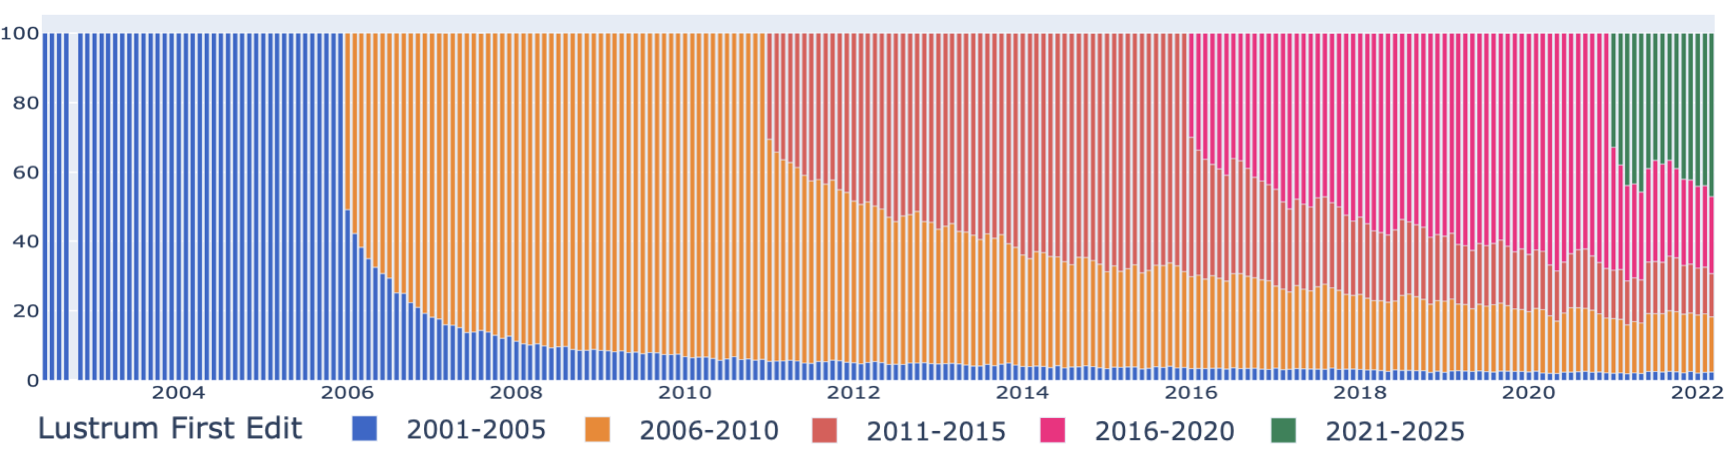
\includegraphics[width=470px]{img/balance.png}
    \setlocalecaption{english}{figure}{Figure}
    \caption{Balance dashboard}
    \label{fig:balance}
\end{figure}

\subsection{Balance implementation}
\label{sec:balance_callback}

The function related to the Balance metric is very similar to the stability one. Thanks to this similarity we take the opportunity to discuss again the basic workflow of each callback.\\
The Dash function, linked to the Dash app, takes as inputs some components' value of the web app layout. In this case, we consider the selected languages, active or very active editors, absolute or percentage values and the timely aggregation of the chart, that can be yearly or monthly; usually, a yearly chart produces more general and meaningful representation of the data and its trends, while a monthly time aggregation favours a discrete and finer-grain data analysis.\\
Then, after having processed the input in order to make them SQL-compliant, we feed them to a parameterized query, that will produce a result set later captured in a Pandas data frame, convenient for the Plotly charts.\\
Finally, we create the figure, in this case a stacked bar chart, that is coded exactly as a common bar chart. We first set the core attributes, like which data column must be placed on the x-axis, y-axis and the \verb#facet_row#, and then the style attributes, like the title, the labels and the size.Once everything is ready, we return the figure to the function responsible for the dynamic layout, displaying it in the appropriate HTML \verb#div#.

\section{Special functions}
\label{sec:special_functions}

The fourth vital sign is called Special functions. It is about editors which hold a certain role that allows them to perform special actions in Wikipedia. In particular, we have two distinct roles: Technical functions and Community coordination functions.\\
Since we have two different classes of functions, we have two different graphs. Two different bar charts that, as the previous vital sign, discriminate the editors based on their generation. The colors are in fact the same.\\
It is evident how the two visualizations look very similar, except for the data distribution. In the dashboards they are paired with a descriptive title.\\

\begin{figure}[h]
    \centering
    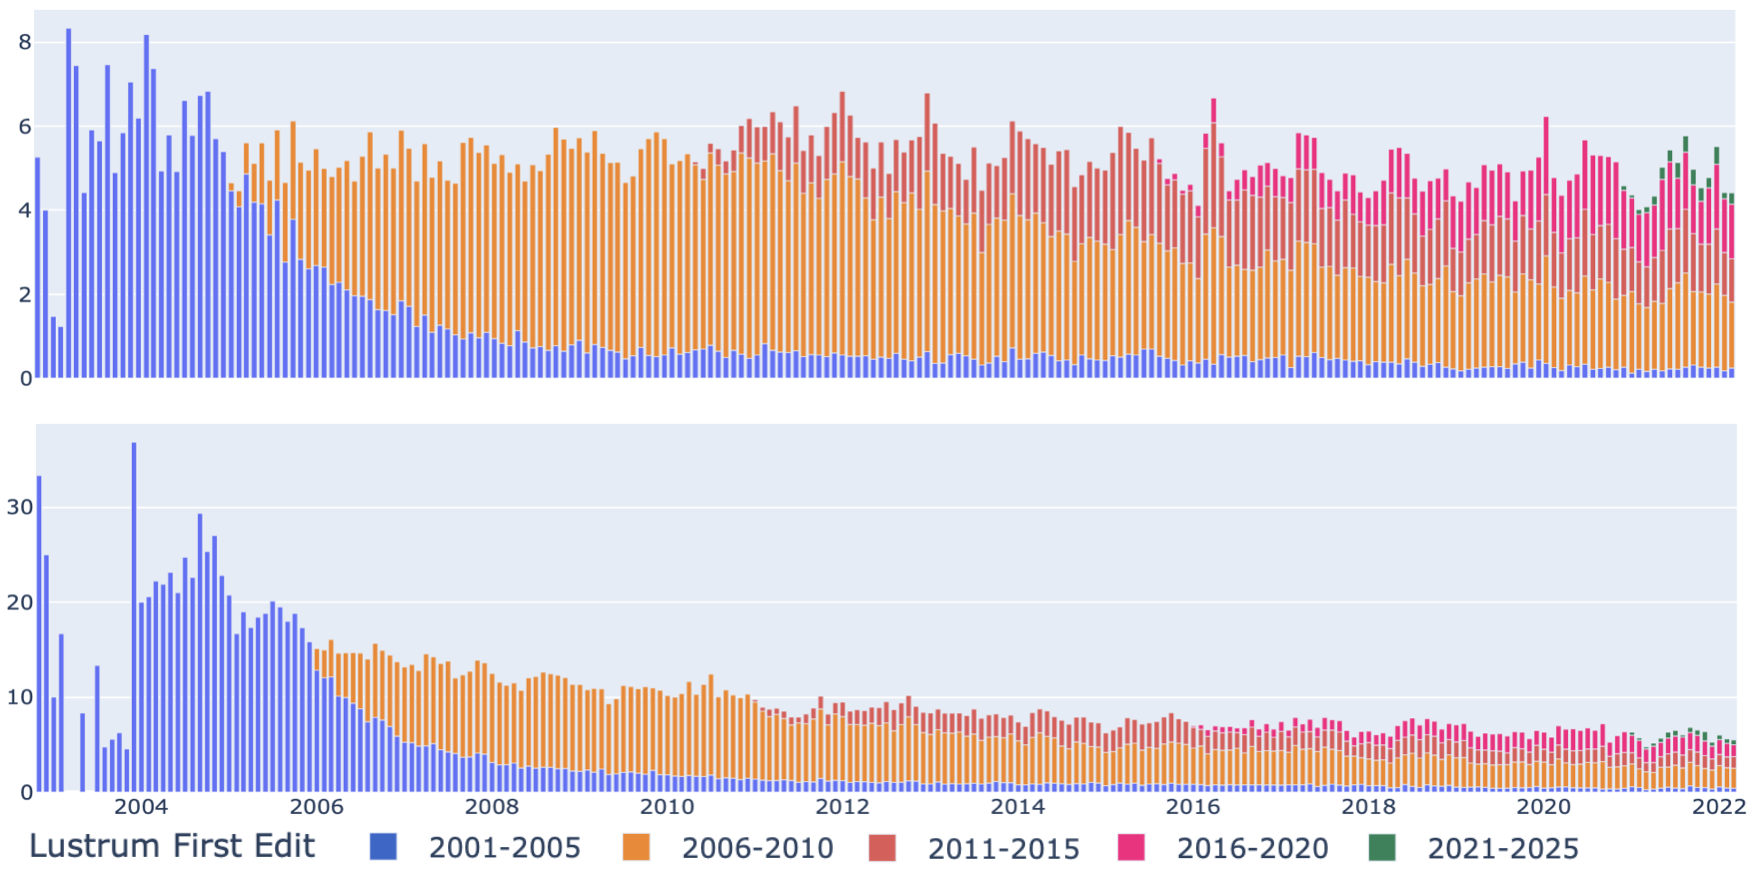
\includegraphics[width=470px]{img/technical_coordinator.png}
    \setlocalecaption{english}{figure}{Figure}
    \caption{Technical and Coordination functions dashboards}
    \label{fig:special_functions}
\end{figure}


\subsection{Special functions implementation}
\label{sec:special_functions_callback}

These two different dashboards have two different callbacks. The two functions work exactly like the other, reading inputs, making a query and creating a figure. To be noted the mechanism with which we return two different graphs in the same layout.\\
We said that the Dash layout contains many HTML components, like the \verb#div# container. There are two of them because some health metric, like Special functions, have two charts to be displayed. In this way we consider this necessity. The functions will output in their respective containers. Also the faceted graph will appear in their intended place.

\section{Admin flags}
\label{sec:admin_flags}

The fifth vital sign is about another kind of specific Wikipedia aspects. This time it is about Administrators. This metric analyzes the distribution in time of editors which hold a position of Wikipedia administrator, with respect to their generation\footnote{The concept of generation is the same for Balance and Specialists}.\\
For this metric the dashboards display three different bar charts.\\
The first one represent the absolute distribution of a certain admin flag over the years. The flag is chosen through the HTML interactive interface.\\
Looking at the charts in Figure \ref{fig:admin} we move to the right to find the second graph: it is a compact view of the first one, since it sums up the editors number discriminating on their generation. The same color as the previous metrics has been kept to enhance the readability and preserve continuity.\\
At the bottom of the Figure \ref{fig:admin}, the third graph is found. It is about the percentage distribution of the previously mentioned admin flag. The title of the graphs changes as the chosen admin flag changes.\\
This time we do not divide the editors in different classes, because we are interested only in the percentage distribution.\\

\begin{figure}[h]
    \centering
    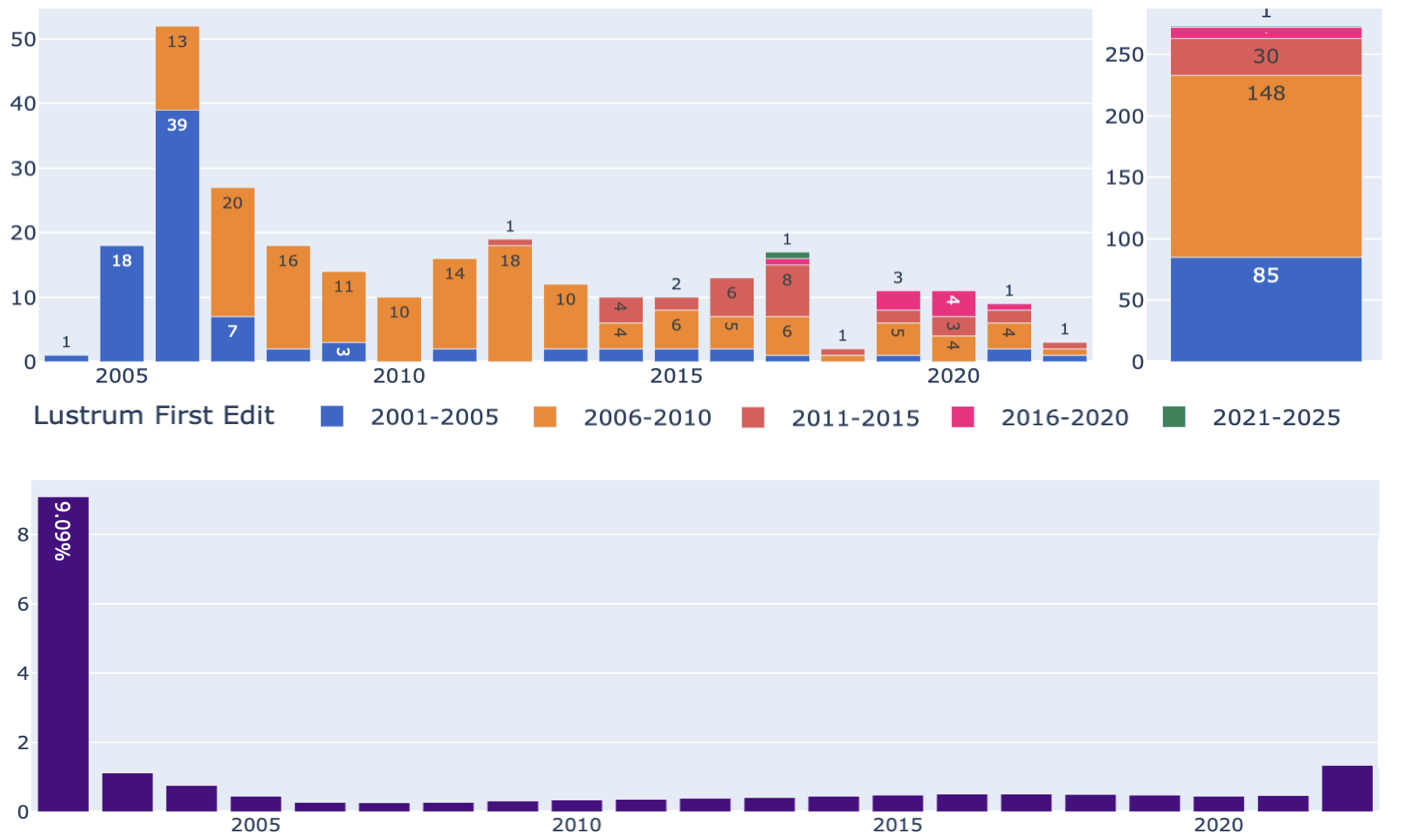
\includegraphics[width=470px]{img/admin.png}
    \setlocalecaption{english}{figure}{Figure}
    \caption{Admin flags dashboards}
    \label{fig:admin}
\end{figure}

\subsection{Admin flags implementation}
\label{sec:admin_flags_callback}

The admin flags' callback has an interesting aspect regarding on which data column we decide to \verb#GROUP BY#. We will not explain how the stacked bar chart are created to avoid time-consuming repetition.\\
We focus on the small chart on the right. It may seem like an extension of the first chart and thus bound to it. But in reality, it is an independent figure.\\
The figure itself is created aside, but its data frame is related to the one used by the first graph.\\ 
For the latter, we retrieve the data about admin editors and we group by the time and by the generation, in order to have the data about different temporal belonging on the same column of the x-axis. Instead, for the second graph we group only by generation, to which we refer as \verb#m2_value# in the python script.
Furthermore, since we are only interested in one-dimension of our data, the absolute values, a new empty data column is created and it is used as the x-axis of this figure, yielding a compact view of our data.
%image? who knows

\section{Global community}
\label{sec:global_community}

The sixth and last vital sign brings the attention to the Global community of Wikipedia. \\
Since Wikipedia is a community project, the participation of each local community to the global one is essential for making their voices heard and learning from others. In this metric we analyze the linguistic origin of the contributions to a certain language community and the contribution of each Wikipedia language community to the global project.\\
This last dashboard has two different charts to satisfy our two different analysis.\\
The first bar chart visualization display the percentage or absolute distribution of all the contributions coming from every available language, towards the chosen language community.\\
For the second analysis we use a peculiar type of graph: a tree-map. As said before, it sums up the individual contribution of each different language community to the global one. Every language is represented as a colorful rectangle whose dimension is proportional to the percentage value of that language contribution to the Meta-Wiki project \cite{meta}. The rectangles also show some additional details like the percentage value and the absolute value. By clicking on one of them there is a little nice animation that expands the whole rectangle, allowing to analyze the small communities too.

\begin{figure}[h]
    \centering
   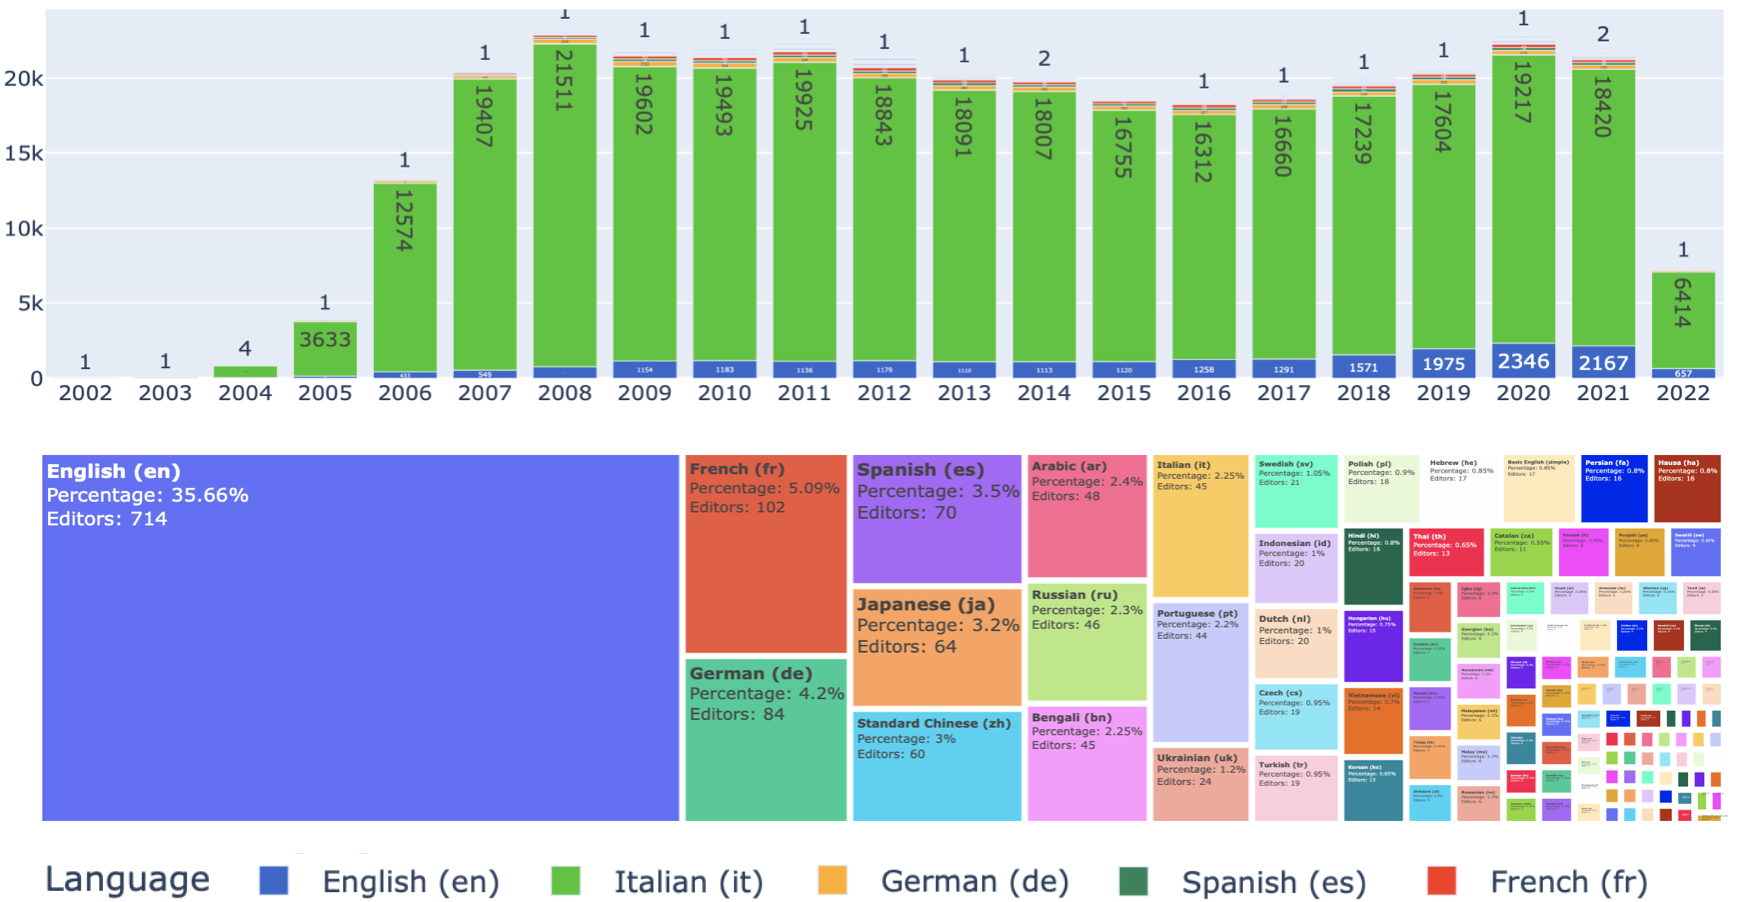
\includegraphics[width=470px]{img/global.png}
    \setlocalecaption{english}{figure}{Figure}
    \caption{Global community participation dashboard}
    \label{fig:global}
\end{figure}


\subsection{Global community implementation}
\label{sec:global_community_callback}

These last dashboards are essential for the project goal since without them we would not have a full picture on the health status of the different communities in Wikipedia. These charts have been realized with a similar code to the others, but this time the colors play an important role since we cannot distinguish different languages in the charts, if not with colors. Unfortunately, there has not been found a way to describe a mapping for every possible language to a unique color since there are simply too many of them. Nonetheless, the results have been considered clearer than what was expected, in particular on the first graph.\\
About the second chart, the tree-map, we used the Plotly sub-module \verb#go#, in a similar way to what was done for the retention visualization. It has been preferred to Plotly Express for its low-level control on the graph figure itself, at the price of a slightly more complex syntax. 
\pagebreak
\lstset{frame=lines}
\lstset{label={lst:code_direct}}
\lstset{basicstyle=\footnotesize}
\lstset{caption=Creating a treemap chart}
\begin{lstlisting}
fig2 = go.Figure()

fig2.add_trace(go.Treemap(
    parents = df2["langcode"],
    labels = df2['language_name'],
    values = df2['m2_count'],
    customdata = df2['perc'],
    text=df2['m2_value'],
    texttemplate = '''<b>%{label} </b><br>Percentage: 
                        %{customdata}%<br>Editors: %{value}<br>''',
    hovertemplate='''<b>%{label} </b><br>Percentage: 
                        %{customdata}%<br>Editors: %{value}<br>
                        %{text}<br><extra></extra>'''))
\end{lstlisting}

A \verb#go.Figure# is created and then we added the tree-map trace, by specifying the common parent for every node (the rectangles) that is the Meta-Wiki topic. Then we set the data column to be textually displayed with the keyword \verb#texttemplate# and to be displayed when we pass over with the mouse pointer with \verb#hovertemplate#. In this way we obtain the visualization in Figure \ref{fig:global} that correctly show us the quantitative distribution of each language communities' contributions to the Meta-Wiki. 

\section{Highlights}
\label{sec:highlights}

In the earlier chapter it was said that the health metrics visualization were paired with automated descriptive labels. In this section we are going to discuss their code and their role. The choice of not talking about them in every single graph was taken due to the fact that the mechanism is the same for every highlight, so we dedicate an entire section to this topic.\\
\\
To enhance graphs' readability we use the Highlights: automated descriptive labels that help us reading the graph and its highest or lowest values. In general, they briefly contextualize the graph and describe what we are looking at.\\
These automatic caption have been coded in a very similar way to the one we used to create the charts: we generate a Pandas data frame with the same technique described before, then we use its data column values to extract the values that will be embedded in some prepared textual statement.
A peculiarity of this mechanism is that the values needed some sort of pre-processing phase: the values had to be casted into a string to be concatenated in the textual statements or the date had to be converted in a user-friendly style like the common ``Month Year" format.\\
\\
In the end, we have at least one function for each graph about the highlights. But to actually place it in the layout we have a dash callback that reads which vital sign has been selected and return the result of the respective highlights function, preserving the dynamicity of the entire layout. In this way, we also ensure the highlights to be up to date with the data selected with the HTML components like the language selected or the time aggregation.

